\documentclass[11pt]{article}

\usepackage{amsthm}
\usepackage{amssymb}
\usepackage{amsmath}
\usepackage{cite}
\usepackage{hyperref}
\usepackage{mathtools}
\usepackage{subcaption}
\usepackage{tikz}
\usepackage{float}
\usepackage{caption}
\usepackage[nottoc]{tocbibind}
\usepackage[english]{babel}
\usepackage[utf8x]{inputenc}
\usepackage[linesnumbered,ruled,lined,boxed,vlined]{algorithm2e}
\usepackage[[deletedmarkup=xout, commentmarkup=footnote]{changes}

\newcommand{\accente}{\`E }

\definechangesauthor[name=Alberto Casagrande, color=red]{ac}

\usetikzlibrary{arrows,automata}
\usetikzlibrary{shapes,snakes}
\usetikzlibrary{arrows.meta}

\captionsetup[figure]{name=Figura}
\captionsetup[table]{name=Tabella}
\renewcommand{\algorithmcfname}{Algoritmo}
\renewcommand\labelitemi{--}

\SetArgSty{textnormal}

\theoremstyle{definition}
\newtheorem{definition}{Definizione}[section]
\newtheorem{example}{Esempio}[section]
\newtheorem{axiom}{Assioma}[section]
\newtheorem*{axiom*}{Assioma}
\newtheorem{observation}{Osservazione}[section]
\newtheorem*{nonobservation}{Osservazione}

\theoremstyle{plain}
\newtheorem{proposition}{Proposizione}[section]
\newtheorem{lemma}{Lemma}[section]
\newtheorem{theorem}{Teorema}[section]
\newtheorem{corollary}{Corollario}[section]

\newcommand{\notimplies}{\mathrel{{\ooalign{\hidewidth$\not\phantom{=}$\hidewidth\cr$\implies$}}}}

\newenvironment{proof2}
{
  \begin{proof}[Dimostrazione]
}
{\end{proof}}

\begin{document}

\renewcommand\contentsname{Indice}
\tableofcontents
\addtocontents{toc}{~\hfill\textbf{Pagina}\par}

\subsection{Grafi}
Il problema che intendiamo affrontare in questo elaborato è descritto con il formalismo della teoria dei grafi. In questa sezione presentiamo un sottoinsieme minimale di definizioni e risultati che ci consentirà di introdurre e trattare la questione.

\subsubsection{Definizione e generalità}
Con le premesse viste sopra possiamo definire un \emph{grafo} come segue:
\begin{definition}
    Sia $V$ un insieme finito non vuoto. Sia $E$ una relazione binaria su $V$. La coppia $G = (V, E)$ è un \emph{grafo diretto} (o \emph{orientato}). Con questa notazione:
    \begin{itemize}
        \item $V$ è l'insieme dei \emph{nodi} (o \emph{vertici});
        \item $E$ è una relazione binaria (in generale non simmetrica) che mette in relazione alcuni dei nodi di $G$.
    \end{itemize}
\end{definition}
\begin{example}
    \begin{figure}[t]
        \centering
        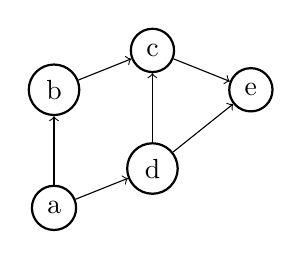
\begin{tikzpicture}[scale=0.5]
            \begin{scope}[every node/.style={circle,thick,draw}]
                \node (a) at (0,0) {a};
                \node (b) at (0,3) {b};
                \node (c) at (2.5,4) {c};
                \node (d) at (2.5,1) {d};
                \node (e) at (5,3) {e};
            \end{scope}

            \begin{scope}
                \path [->] (a) edge node {} (b);
                \path [->] (b) edge node {} (c);
                \path [->] (a) edge node {} (d);
                \path [->] (d) edge node {} (c);
                \path [->] (d) edge node {} (e);
                \path [->] (c) edge node {} (e);
            \end{scope}
            \end{tikzpicture}
        \caption{Rappresentazione grafica di un grafo diretto}
        \label{fig:graph}
    \end{figure}
    Il grafo di Figura \ref{fig:graph} è descritto dalla coppia
    \begin{itemize}
        \item $V = \{a,b,c,d,e\}$
        \item $E = \{(a,b), (a,d), (b,c), (d,c), (c,e), (d,e)\}$
    \end{itemize}
\end{example}
Nel seguito utilizzeremo ampiamente la seguente terminologia:
\begin{definition}
    Sia $G = (V,E)$ un grafo diretto. Consideriamo un arco $(u,v) \in E$. In questo caso $u$ è la \emph{sorgente} dell'arco, mentre $v$ è la \emph{destinazione}. Se il numero di archi uscenti da un nodo è zero, allora tale nodo  è un \emph{pozzo} (dall'inglese \emph{sink}).
\end{definition}

\subsubsection{Componenti fortemente connesse}
Come abbiamo visto sopra, un grafo diretto è un insieme di elementi (i \emph{nodi}) accoppiato con un insieme di relazioni tra questi elementi (gli \emph{archi}). \accente naturale associare questo concetto all'idea di percorso: ogni grafo è definito da un insieme di nodi ed un insieme di \emph{cammini} che consentono di spostarsi da un nodo ad un altro. La seguente definizione sorge in modo spontaneo da questa interpretazione:
\begin{definition}
    Sia $G = (V, E)$ un grafo diretto. Siano $u,v \in V$. $v$ \emph{è raggiungibile} da $u$, o in alternativa \emph{esiste un cammino} da $u$ a $v$, o ancora $u E^{*} v$, se esiste una sequenza finita di nodi $\displaystyle \{x_n\}_{n \in \{0,\dots,K\}}$, tale che $x_0 = u, x_K = v, x_n E x_{n+1}$.
\end{definition}
L'esistenza di un cammino tra nodi fornisce un criterio immediato per partizionare un grafo in gruppi di nodi. Diamo innanzitutto la seguente definizione:
\begin{definition}
    Un grafo diretto $(V,E)$ è \emph{fortemente connesso} se per ogni coppia di nodi $v_1, v_2 \in V$ esiste un cammino da $v_1$ a $v_2$, cioè $v_1 E^{*} v_2$.
\end{definition}
Allora possiamo individuare i sottografi massimali (cioè la ripartizione del grafo in sottografi che consente di minimizzare il numero di sottografi) fortemente connessi (\hspace*{-0.1cm}\cite[Appendice B]{clrs}):
\begin{definition}
    Le \emph{componenti fortemente connesse} (\emph{strongly connected components}, \emph{SCC}) di un grafo diretto sono i sottografi che compongono la ripartizione (massimale) del grafo in sottografi fortemente connessi.
\end{definition}
\begin{example}
    \begin{figure}[t]
        \centering
        \begin{tikzpicture}[scale=0.5]
            \begin{scope}[every node/.style={circle,thick,draw}]
                \node (a) at (0,0) {a};
                \node (b) at (0,3) {b};
                \node (c) at (2.5,4) {c};
                \node (d) at (2.5,1) {d};
                \node (e)[diamond] at (5,3) {e};
            \end{scope}

            \begin{scope}
                \path [->] (a) edge node {} (b);
                \path [->] (b) edge node {} (c);
                \path [->] (d) edge node {} (a);
                \path [->] (c) edge node {} (d);
                \path [->] (d) edge node {} (e);
                \path [->] (c) edge node {} (e);
            \end{scope}
            \end{tikzpicture}
        \caption{SCC di un grafo diretto}
        \label{fig:graph_cfc_1}
    \end{figure}
    Nel grafo di Figura \ref{fig:graph_cfc_1} le SCC sono rappresentate con forme diverse: $\{a,b,c,d\}, \{e\}$.
\end{example}
Il partizionamento dei nodi in SCC è definito come segue:
\begin{definition} \label{def:scc_partition}
    Sia $G = (V, E)$ un grafo diretto. Il grafo $G^{\superscc} = (V^{\superscc}, E^{\superscc})$, dove:
    \begin{itemize}
        \item $V^{\superscc} = \{C \mid \,C$ è una SCC$\}$;
        \item $E^{\superscc} = \{(A,B) \in V^{\superscc} \times V^{\superscc} \mid A \neq B, \exists m \in A, n \in B, m E n\}$
    \end{itemize}
    è il partizionamento del grafo iniziale in SCC.
\end{definition}
Riportiamo la seguente proprietà immediata:
\begin{proposition}
    Sia $G^{\superscc}$ il grafo delle SCC di un grafo $G$ generico. Allora $G^{\superscc}$ è aciclico.
\end{proposition}
\begin{proof2}
    Supponiamo per assurdo che in $G^{\superscc}$ esista un ciclo. Allora tutti i nodi di $V^{\superscc}$ facenti parte del ciclo sono mutuamente raggiungibili (percorrendo il ciclo). Quindi tutti i nodi fanno parte della stessa SCC, ma questo è assurdo.
\end{proof2}
\begin{example}
    \begin{figure}[t]
        \centering
        \begin{subfigure}{.45\textwidth}
          \centering
          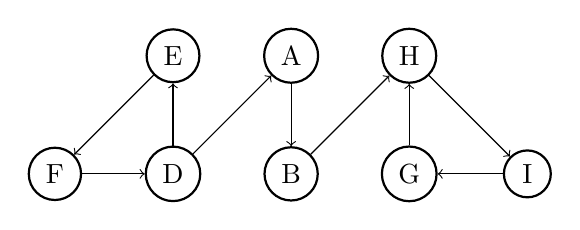
\begin{tikzpicture}[scale=0.5]
            \begin{scope}[every node/.style={circle,thick,draw}]
                \node (A) at (0,3) {A};
                \node (B) at (0,0) {B};

                \node (D) at (-3,0) {D};
                \node (E) at (-3,3) {E};
                \node (F) at (-6,0) {F};

                \node (G) at (3,0) {G};
                \node (H) at (3,3) {H};
                \node (I) at (6,0) {I};
            \end{scope}

            \begin{scope}
                \path [->] (A) edge node {} (B);

                \path [->] (E) edge node {} (F);
                \path [->] (F) edge node {} (D);
                \path [->] (D) edge node {} (E);

                \path [->] (G) edge node {} (H);
                \path [->] (H) edge node {} (I);
                \path [->] (I) edge node {} (G);

                \path [->] (D) edge node {} (A);
                \path [->] (B) edge node {} (H);
            \end{scope}
            \end{tikzpicture}
          \caption{Un grafo}
        \end{subfigure}
        \hfill
        \begin{subfigure}{.45\textwidth}
          \centering
          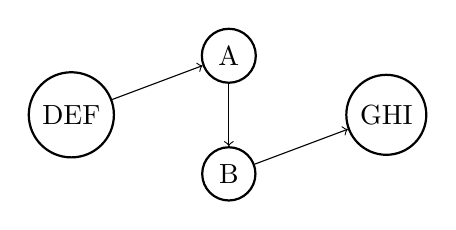
\begin{tikzpicture}[scale=0.5]
            \begin{scope}[every node/.style={circle,thick,draw}]
                \node (A) at (0,3) {A};
                \node (B) at (0,0) {B};

                \node (DEF) at (-4,1.5) {DEF};

                \node (GHI) at (4,1.5) {GHI};
            \end{scope}
                \path [->] (A) edge node {} (B);
                \path [->] (DEF) edge node {} (A);
                \path [->] (B) edge node {} (GHI);
            \begin{scope}

            \end{scope}
            \end{tikzpicture}
          \caption{Corrispondente grafo delle SCC}
        \end{subfigure}
        \caption{Un grafo ed il corrispondente grafo delle SCC}
        \label{fig:graph_cfc_2}
    \end{figure}
    La Figura \ref{fig:graph_cfc_2}.a rappresenta un grafo diretto generico, la Figura \ref{fig:graph_cfc_2}.b rappresenta il suo grafo delle componenti fortemente connesse associato.
\end{example}
Dato un grafo diretto generico possiamo determinare la ripartizione in SCC dei suoi nodi sfruttando un algoritmo avente complessità lineare $\Theta(|V| + |E|)$ \cite{tarjan}. L'algoritmo non verrà trattato in questo elaborato.\\

\subsubsection{Visita in profondità}
Delle due metodologie prevalenti per l'esplorazione di un grafo, \emph{visita in ampiezza} (\emph{Breadth-First-Search}, abbreviato in BFS) e \emph{visita in profondità} (\emph{Depth-First-Search}, abbreviato in DFS), in questo lavoro ci interessiamo alla seconda. Come dice il nome, questa tecnica consiste nella visita esaustiva di tutti i figli di un nodo, prima di passare agli altri nodi sullo stesso livello. Riportiamo lo pseudocodice da \cite{clrs}, leggermente modificato:\\
\begin{algorithm}[H]
    \label{alg:dfs}
    \KwData{$G = (V,E)$}
    \caption{DFS}
    \SetAlgoLined
    \SetKwProg{Fn}{function}{:}{end}
    \Fn{\textup{dsf-visit}($G = (V,E), n,$ time)}{
        n.color = GRAY\;
        \ForAll{$m \mid (nEm \land m.$color = WHITE)}{
            time = dfs-visit($G, m,$ time)\;
        }
        n.finishing-time = time\;
        n.color = BLACK\;
        time = time+1\;
        \Return{time}\;
    }
    \Begin{
        \ForAll{$n \in V$}{
            n.color = WHITE\;
        }

        time = 0\;
        \While{$\exists n \in V \mid n.color ==$ WHITE}{
            time = dfs-visit($G,n,$ time)\;
        }
    }
\end{algorithm}
L'attributo \emph{color} dei nodi del grafo consente di distinguere tra quei nodi che sono già stati visitati in modo esauriente (colore nero), quelli per cui è in corso una visita in profondità (colore grigio) e quelli non ancora esaminati dall'algoritmo (colore bianco). Si osservi che la colorazione dei nodi non è solamente accessoria, ma fornisce un meccanismo per evitare un loop infinito nel caso in cui il grafo contenga un ciclo.

Oltre alla colorazione dei nodi, l'algoritmo imposta l'attributo \emph{finishing-time} per ogni nodo, ovvero l'istante di tempo (a partire da \emph{time} $= 0$) in cui è stata terminata la visita esaustiva in profondità per tale nodo. Nello pseudocodice completo vengono considerati altri due attributi: \emph{starting-time} e \emph{parent}. Questi ultimi tre attributi forniscono alcune importanti proprietà all'algoritmo di visita in profondità, che non saranno approfondite in questo lavoro (si vedano \emph{Parenthesis theorem}, \emph{White-path theorem} in \cite{clrs}).

L'attributo \emph{finishing-time} è sufficiente per alcune applicazioni che saranno esposte nelle sezioni seguenti.

\subsection{Grafi}
Il problema che intendiamo affrontare in questo elaborato è descritto con il formalismo della teoria dei grafi. In questa sezione presentiamo un sottoinsieme minimale di definizioni e risultati che ci consentirà di introdurre e trattare la questione.

\subsubsection{Definizione e generalità}
Con le premesse viste sopra possiamo definire un \emph{grafo} come segue:
\begin{definition}
    Sia $V$ un insieme finito non vuoto. Sia $E$ una relazione binaria su $V$. La coppia $G = (V, E)$ è un \emph{grafo diretto} (o \emph{orientato}). Con questa notazione:
    \begin{itemize}
        \item $V$ è l'insieme dei \emph{nodi} (o \emph{vertici});
        \item $E$ è una relazione binaria (in generale non simmetrica) che mette in relazione alcuni dei nodi di $G$.
    \end{itemize}
\end{definition}
\begin{example}
    \begin{figure}[t]
        \centering
        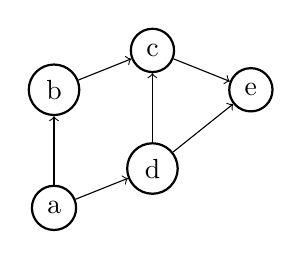
\begin{tikzpicture}[scale=0.5]
            \begin{scope}[every node/.style={circle,thick,draw}]
                \node (a) at (0,0) {a};
                \node (b) at (0,3) {b};
                \node (c) at (2.5,4) {c};
                \node (d) at (2.5,1) {d};
                \node (e) at (5,3) {e};
            \end{scope}

            \begin{scope}
                \path [->] (a) edge node {} (b);
                \path [->] (b) edge node {} (c);
                \path [->] (a) edge node {} (d);
                \path [->] (d) edge node {} (c);
                \path [->] (d) edge node {} (e);
                \path [->] (c) edge node {} (e);
            \end{scope}
            \end{tikzpicture}
        \caption{Rappresentazione grafica di un grafo diretto}
        \label{fig:graph}
    \end{figure}
    Il grafo di Figura \ref{fig:graph} è descritto dalla coppia
    \begin{itemize}
        \item $V = \{a,b,c,d,e\}$
        \item $E = \{(a,b), (a,d), (b,c), (d,c), (c,e), (d,e)\}$
    \end{itemize}
\end{example}
Nel seguito utilizzeremo ampiamente la seguente terminologia:
\begin{definition}
    Sia $G = (V,E)$ un grafo diretto. Consideriamo un arco $(u,v) \in E$. In questo caso $u$ è la \emph{sorgente} dell'arco, mentre $v$ è la \emph{destinazione}. Se il numero di archi uscenti da un nodo è zero, allora tale nodo  è un \emph{pozzo} (dall'inglese \emph{sink}).
\end{definition}

\subsubsection{Componenti fortemente connesse}
Come abbiamo visto sopra, un grafo diretto è un insieme di elementi (i \emph{nodi}) accoppiato con un insieme di relazioni tra questi elementi (gli \emph{archi}). \accente naturale associare questo concetto all'idea di percorso: ogni grafo è definito da un insieme di nodi ed un insieme di \emph{cammini} che consentono di spostarsi da un nodo ad un altro. La seguente definizione sorge in modo spontaneo da questa interpretazione:
\begin{definition}
    Sia $G = (V, E)$ un grafo diretto. Siano $u,v \in V$. $v$ \emph{è raggiungibile} da $u$, o in alternativa \emph{esiste un cammino} da $u$ a $v$, o ancora $u E^{*} v$, se esiste una sequenza finita di nodi $\displaystyle \{x_n\}_{n \in \{0,\dots,K\}}$, tale che $x_0 = u, x_K = v, x_n E x_{n+1}$.
\end{definition}
L'esistenza di un cammino tra nodi fornisce un criterio immediato per partizionare un grafo in gruppi di nodi. Diamo innanzitutto la seguente definizione:
\begin{definition}
    Un grafo diretto $(V,E)$ è \emph{fortemente connesso} se per ogni coppia di nodi $v_1, v_2 \in V$ esiste un cammino da $v_1$ a $v_2$, cioè $v_1 E^{*} v_2$.
\end{definition}
Allora possiamo individuare i sottografi massimali (cioè la ripartizione del grafo in sottografi che consente di minimizzare il numero di sottografi) fortemente connessi (\hspace*{-0.1cm}\cite[Appendice B]{clrs}):
\begin{definition}
    Le \emph{componenti fortemente connesse} (\emph{strongly connected components}, \emph{SCC}) di un grafo diretto sono i sottografi che compongono la ripartizione (massimale) del grafo in sottografi fortemente connessi.
\end{definition}
\begin{example}
    \begin{figure}[t]
        \centering
        \begin{tikzpicture}[scale=0.5]
            \begin{scope}[every node/.style={circle,thick,draw}]
                \node (a) at (0,0) {a};
                \node (b) at (0,3) {b};
                \node (c) at (2.5,4) {c};
                \node (d) at (2.5,1) {d};
                \node (e)[diamond] at (5,3) {e};
            \end{scope}

            \begin{scope}
                \path [->] (a) edge node {} (b);
                \path [->] (b) edge node {} (c);
                \path [->] (d) edge node {} (a);
                \path [->] (c) edge node {} (d);
                \path [->] (d) edge node {} (e);
                \path [->] (c) edge node {} (e);
            \end{scope}
            \end{tikzpicture}
        \caption{SCC di un grafo diretto}
        \label{fig:graph_cfc_1}
    \end{figure}
    Nel grafo di Figura \ref{fig:graph_cfc_1} le SCC sono rappresentate con forme diverse: $\{a,b,c,d\}, \{e\}$.
\end{example}
Il partizionamento dei nodi in SCC è definito come segue:
\begin{definition} \label{def:scc_partition}
    Sia $G = (V, E)$ un grafo diretto. Il grafo $G^{\superscc} = (V^{\superscc}, E^{\superscc})$, dove:
    \begin{itemize}
        \item $V^{\superscc} = \{C \mid \,C$ è una SCC$\}$;
        \item $E^{\superscc} = \{(A,B) \in V^{\superscc} \times V^{\superscc} \mid A \neq B, \exists m \in A, n \in B, m E n\}$
    \end{itemize}
    è il partizionamento del grafo iniziale in SCC.
\end{definition}
Riportiamo la seguente proprietà immediata:
\begin{proposition}
    Sia $G^{\superscc}$ il grafo delle SCC di un grafo $G$ generico. Allora $G^{\superscc}$ è aciclico.
\end{proposition}
\begin{proof2}
    Supponiamo per assurdo che in $G^{\superscc}$ esista un ciclo. Allora tutti i nodi di $V^{\superscc}$ facenti parte del ciclo sono mutuamente raggiungibili (percorrendo il ciclo). Quindi tutti i nodi fanno parte della stessa SCC, ma questo è assurdo.
\end{proof2}
\begin{example}
    \begin{figure}[t]
        \centering
        \begin{subfigure}{.45\textwidth}
          \centering
          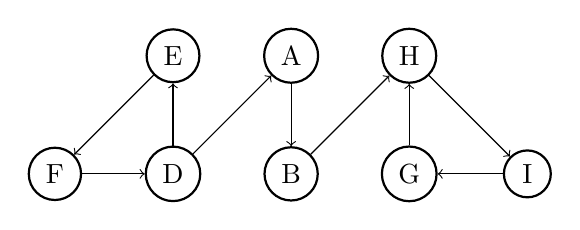
\begin{tikzpicture}[scale=0.5]
            \begin{scope}[every node/.style={circle,thick,draw}]
                \node (A) at (0,3) {A};
                \node (B) at (0,0) {B};

                \node (D) at (-3,0) {D};
                \node (E) at (-3,3) {E};
                \node (F) at (-6,0) {F};

                \node (G) at (3,0) {G};
                \node (H) at (3,3) {H};
                \node (I) at (6,0) {I};
            \end{scope}

            \begin{scope}
                \path [->] (A) edge node {} (B);

                \path [->] (E) edge node {} (F);
                \path [->] (F) edge node {} (D);
                \path [->] (D) edge node {} (E);

                \path [->] (G) edge node {} (H);
                \path [->] (H) edge node {} (I);
                \path [->] (I) edge node {} (G);

                \path [->] (D) edge node {} (A);
                \path [->] (B) edge node {} (H);
            \end{scope}
            \end{tikzpicture}
          \caption{Un grafo}
        \end{subfigure}
        \hfill
        \begin{subfigure}{.45\textwidth}
          \centering
          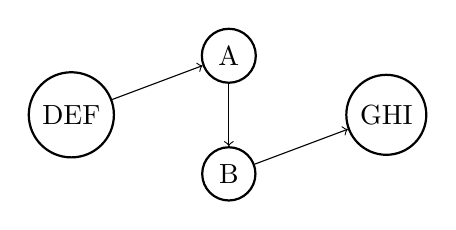
\begin{tikzpicture}[scale=0.5]
            \begin{scope}[every node/.style={circle,thick,draw}]
                \node (A) at (0,3) {A};
                \node (B) at (0,0) {B};

                \node (DEF) at (-4,1.5) {DEF};

                \node (GHI) at (4,1.5) {GHI};
            \end{scope}
                \path [->] (A) edge node {} (B);
                \path [->] (DEF) edge node {} (A);
                \path [->] (B) edge node {} (GHI);
            \begin{scope}

            \end{scope}
            \end{tikzpicture}
          \caption{Corrispondente grafo delle SCC}
        \end{subfigure}
        \caption{Un grafo ed il corrispondente grafo delle SCC}
        \label{fig:graph_cfc_2}
    \end{figure}
    La Figura \ref{fig:graph_cfc_2}.a rappresenta un grafo diretto generico, la Figura \ref{fig:graph_cfc_2}.b rappresenta il suo grafo delle componenti fortemente connesse associato.
\end{example}
Dato un grafo diretto generico possiamo determinare la ripartizione in SCC dei suoi nodi sfruttando un algoritmo avente complessità lineare $\Theta(|V| + |E|)$ \cite{tarjan}. L'algoritmo non verrà trattato in questo elaborato.\\

\subsubsection{Visita in profondità}
Delle due metodologie prevalenti per l'esplorazione di un grafo, \emph{visita in ampiezza} (\emph{Breadth-First-Search}, abbreviato in BFS) e \emph{visita in profondità} (\emph{Depth-First-Search}, abbreviato in DFS), in questo lavoro ci interessiamo alla seconda. Come dice il nome, questa tecnica consiste nella visita esaustiva di tutti i figli di un nodo, prima di passare agli altri nodi sullo stesso livello. Riportiamo lo pseudocodice da \cite{clrs}, leggermente modificato:\\
\begin{algorithm}[H]
    \label{alg:dfs}
    \KwData{$G = (V,E)$}
    \caption{DFS}
    \SetAlgoLined
    \SetKwProg{Fn}{function}{:}{end}
    \Fn{\textup{dsf-visit}($G = (V,E), n,$ time)}{
        n.color = GRAY\;
        \ForAll{$m \mid (nEm \land m.$color = WHITE)}{
            time = dfs-visit($G, m,$ time)\;
        }
        n.finishing-time = time\;
        n.color = BLACK\;
        time = time+1\;
        \Return{time}\;
    }
    \Begin{
        \ForAll{$n \in V$}{
            n.color = WHITE\;
        }

        time = 0\;
        \While{$\exists n \in V \mid n.color ==$ WHITE}{
            time = dfs-visit($G,n,$ time)\;
        }
    }
\end{algorithm}
L'attributo \emph{color} dei nodi del grafo consente di distinguere tra quei nodi che sono già stati visitati in modo esauriente (colore nero), quelli per cui è in corso una visita in profondità (colore grigio) e quelli non ancora esaminati dall'algoritmo (colore bianco). Si osservi che la colorazione dei nodi non è solamente accessoria, ma fornisce un meccanismo per evitare un loop infinito nel caso in cui il grafo contenga un ciclo.

Oltre alla colorazione dei nodi, l'algoritmo imposta l'attributo \emph{finishing-time} per ogni nodo, ovvero l'istante di tempo (a partire da \emph{time} $= 0$) in cui è stata terminata la visita esaustiva in profondità per tale nodo. Nello pseudocodice completo vengono considerati altri due attributi: \emph{starting-time} e \emph{parent}. Questi ultimi tre attributi forniscono alcune importanti proprietà all'algoritmo di visita in profondità, che non saranno approfondite in questo lavoro (si vedano \emph{Parenthesis theorem}, \emph{White-path theorem} in \cite{clrs}).

L'attributo \emph{finishing-time} è sufficiente per alcune applicazioni che saranno esposte nelle sezioni seguenti.


\renewcommand\refname{Bibliografia}
\bibliographystyle{plain}
\bibliography{bibliography}

\end{document}
